\par\Needspace{10\baselineskip}
\section{曲面积分}
\label{sec:analysis-surface-integration}

路径积分按长度累计细线上的量，曲面积分则按面积累计薄片上的量。
这里有两个不同的被积对象：标量函数$h:S\to\mathbb R$给出每单位面积的密度，
向量场$\bm F:S\to\mathbb R^3$给出空间中各点处有大小和方向的作用。
前者乘面积得到质量等总量；后者先取法向分量，再乘面积得到穿过曲面的通量。
二者都需要由参数化求出面积元，但只有通量需要选定法向。
本节先建立共同的曲面几何，再分别研究两类积分的定义、可积性、性质和计算。
全部积分采用勒贝格积分；参数曲面、面积元和通量的标准构造可参考\scite{math-openstax-calculus3}。

\subsection{参数曲面与面积}

空间中的曲面通常不能用一个平面区域直接代替，但可以用两个参数标记曲面上的点。
参数化的作用是把曲面上的累计转回二维参数域，同时用面积权重补偿曲面的倾斜和伸缩。

\subsubsection{曲面的参数化}

\paragraph{正则曲面片}

曲面的参数化是向量值映射：输入两个实数，输出三个空间坐标。
为了让它描述一张面，需要两个参数方向真正独立，并避免把同一片面重复计算。

\begin{definition}[正则参数曲面片]
\label{def:analysis-regular-surface-patch}
设$E\subseteq\mathbb R^2$是有界闭区域，$E=\overline{E^\circ}$且二维勒贝格测度$m_2(\partial E)=0$。
设$\bm r$在$E$的一个开邻域内是$C^1$映射，写成
\[
 \bm r(u,v)=(x(u,v),y(u,v),z(u,v))^\top\in\mathbb R^3.
\]
若不同参数只有在都属于$\partial E$时才允许表示同一点，
且两个偏导向量$\bm r_u,\bm r_v$在$E^\circ$上处处线性无关，则称$\bm r$为一个正则曲面片的参数化，曲面片记为$S=\bm r(E)$。
参数边界允许产生接缝或退化点；这些边界部分按零曲面面积处理。
\end{definition}

这里两个切向量线性无关，是指对任意实数$\alpha,\beta$，
$\alpha\bm r_u+\beta\bm r_v=\bm0$只有在$\alpha=\beta=0$时才成立。

固定$v$而改变$u$得到一条参数曲线，它的速度是$\bm r_u$；固定$u$得到的另一条参数曲线的速度是$\bm r_v$。
二者张成曲面的切平面。这里$\bm r_u,\bm r_v$都是三维向量，
并非某个标量函数的两个偏导数。
例如$\bm r(u,v)=(u,v,u+v)^\top$、$E=[0,1]^2$描述平面$z=x+y$上的一块平行四边形，
两个切向量分别为$(1,0,1)^\top$和$(0,1,1)^\top$。

\paragraph{叉积}

小参数矩形的两条边近似映为$\bm r_u\Delta u$和$\bm r_v\Delta v$。
要求它们张成的平行四边形面积，需要一个同时记录面积和垂直方向的向量运算。
对$\bm a,\bm b\in\mathbb R^3$，定义叉积
\[
 \bm a\times\bm b
 =(a_2b_3-a_3b_2,\ a_3b_1-a_1b_3,\ a_1b_2-a_2b_1)^\top.
\]
它垂直于$\bm a,\bm b$，长度等于两向量张成的平行四边形面积，交换次序则变号。
因此正则性也可以写成$\bm r_u\times\bm r_v\ne\bm0$，
小曲面片的面积近似为$\lVert\bm r_u\times\bm r_v\rVert_2\Delta u\Delta v$。

\subsubsection{曲面面积的表示}

\paragraph{面积元与面积测度}

参数域上的面积$\mathrm du\,\mathrm dv$与曲面上的实际面积通常不同。
把刚才得到的局部面积比作为权重，就能把二维勒贝格测度转成曲面上的面积测度。

\begin{definition}[曲面面积测度]
\label{def:analysis-surface-area-measure}
在上述曲面片上，记$J_S(u,v)=\lVert\bm r_u\times\bm r_v\rVert_2$。
若$A\subseteq S$的原像$\bm r^{-1}(A)\cap E$勒贝格可测，则称$A$为曲面可测集，定义
\[
 \sigma_S(A)=\iint_E\bm1_A(\bm r(u,v))J_S(u,v)\,\mathrm du\,\mathrm dv.
\]
曲面面积元记为$\mathrm dS$，参数表示为
\[
 \mathrm dS=J_S(u,v)\,\mathrm du\,\mathrm dv,
 \qquad \operatorname{area}(S)=\sigma_S(S).
\]
\end{definition}

原像保留集合的补、交和并，而右侧是非负权重下的勒贝格积分，
所以这些曲面可测集构成$\sigma$代数，$\sigma_S$在其上可数可加。
$J_S$在紧集$E$上连续有界，且$m_2(E)<\infty$，故这里的曲面片面积有限。
参数边界的二维测度为零，不贡献面积；边界接缝上的重复参数也不重复累计正面积部分。
前面的斜平面片有$\bm r_u\times\bm r_v=(-1,-1,1)^\top$，
故$J_S=\sqrt3$，其面积为$\sqrt3$，而参数正方形的面积为$1$。


图~\ref{fig:analysis-process-surface-area-stretch}将参数小块与实际斜面小块对应起来，解释叉积长度校正的是哪一个面积。
\begin{figure*}[!htbp]
 \centering
 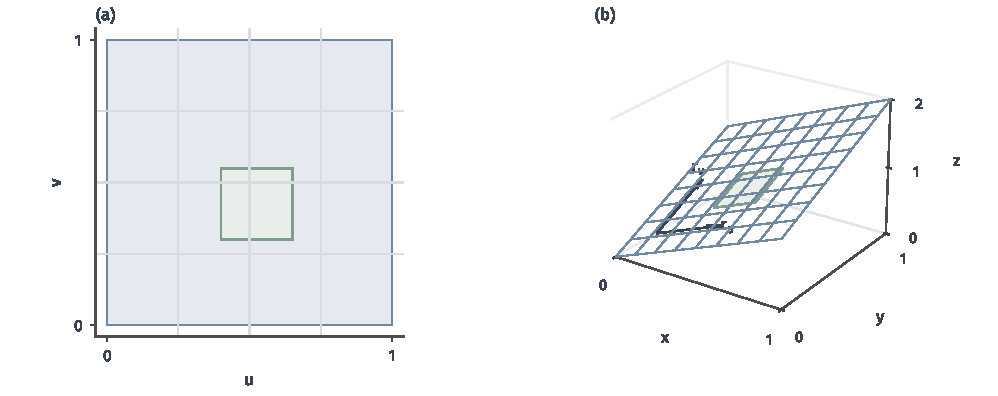
\includegraphics[width=169.0mm]{figures/01-mathematical-preliminaries-upper/01-mathematical-language-combinatorics-analysis-optimization/matplotlib/chapter3-concept-processes/surface-area-stretch.pdf}
 \caption{参数化$r(u,v)=(u,v,u+v)^\top$把单位正方形映为斜平面片，绿色块为同一参数子区间及其像。两切向量$r_u=(1,0,1)^\top$、$r_v=(0,1,1)^\top$在右侧按$0.4$倍画出，叉积长度为$\sqrt3$。每个参数面积都放大$\sqrt3$倍，故不能把$\mathrm du\,\mathrm dv$直接当成$\mathrm dS$。}
 \label{fig:analysis-process-surface-area-stretch}
\end{figure*}

\paragraph{重参数化}

同一块面可以用不同参数标记。要让上面的面积描述曲面本身，
还需证明更换单次覆盖的参数后，面积权重恰好抵消参数域的面积变化。

\begin{theorem}[重参数化下的面积元]
\label{thm:analysis-surface-reparameterization}
设$\bm r:E\to S$满足上述条件，$T:\widetilde E\to E$是参数域之间的双射，
在闭域的开邻域内为$C^1$映射，并在内部是$C^1$微分同胚。
若$\widetilde{\bm r}=\bm r\circ T$仍满足曲面片条件，则
\[
 \begin{aligned}
 \widetilde{\bm r}_\xi\times\widetilde{\bm r}_\eta
 &=\det\bm J_T\,(\bm r_u\times\bm r_v)\circ T,\\
 \widetilde J_S&=(J_S\circ T)|\det\bm J_T|.
 \end{aligned}
\]
两组参数由此给出同一面积测度。
\end{theorem}

\begin{proof}
链式法则给出$\widetilde{\bm r}_\xi=\bm r_u u_\xi+\bm r_v v_\xi$和
$\widetilde{\bm r}_\eta=\bm r_u u_\eta+\bm r_v v_\eta$，其中右端各量在$T(\xi,\eta)$处取值。
利用叉积的双线性、$\bm a\times\bm a=\bm0$和交换次序变号，得到
\[
 \widetilde{\bm r}_\xi\times\widetilde{\bm r}_\eta
 =(u_\xi v_\eta-v_\xi u_\eta)(\bm r_u\times\bm r_v)\circ T.
\]
取长度得到第二式。将它代入任一可测集$A$的面积定义，
二维勒贝格积分的换元公式便把新参数下的积分变回原积分。
\end{proof}

行列式的绝对值保证面积非负；行列式本身的符号则记录参数次序是否翻转，
后面选取通量的法向时还会使用这一信息。
若参数在正面积范围内重复覆盖，参数积分会重复累计，不能直接把它当作单次曲面面积。

\paragraph{分片曲面}

球面、封闭边界或带折角的曲面可能需要多张参数片描述。
本节处理有限分片的情形：各片内部不重叠，交接部分在相邻曲面片中面积均为零，
整个曲面的面积测度由各片面积测度相加。
这样曲面面积和后面的面积积分都可以逐片计算，不需在接缝上补加一项。
无界曲面或不能由这里的有限正则片覆盖的曲面，还需另外处理覆盖和可积性条件。

\subsection{第一类曲面积分}

给定曲面以后，先考虑标量函数$h$在曲面上的累计。
面积测度已经确定了每块薄片的权重，因此可以直接沿用前面建立的测度积分。

\subsubsection{积分的定义和可积性}

\paragraph{按面积的积分}

把面密度乘小片面积再相加，提示我们应当对面积测度积分。
下面的定义既包含连续密度，也允许有跳跃或仅可测的密度。

\begin{definition}[第一类曲面积分]
\label{def:analysis-scalar-surface-integral}
设$h$是$S$上的可测标量函数。
当$h\geq0$时，定义它的\term{第一类曲面积分}（scalar surface integral）为
\begin{equation}
 \int_Sh\,\mathrm dS
 =\iint_Eh(\bm r(u,v))J_S(u,v)\,\mathrm du\,\mathrm dv.
 \label{eq:analysis-scalar-surface-integral}
\end{equation}
该值允许为$+\infty$。一般实值$h$在$\int_S|h|\,\mathrm dS<\infty$时称为曲面可积，
其积分按正、负部分之差定义，仍满足上式。
\end{definition}

取$h=1$得到面积，取非负面密度得到质量。
在前面的单位参数斜平面片上，常数密度$h=2$给出
\[
 \int_S2\,\mathrm dS=\int_0^1\int_0^1 2\sqrt3\,\mathrm du\,\mathrm dv=2\sqrt3.
\]
这一累计不使用法向，因此把曲面的朝向反过来不会改变结果。

\paragraph{可积性的要求}

积分是否有限，取决于函数大小和曲面面积权重共同作用后的累计。
由定义，$h$曲面可积当且仅当参数函数可测且
\[
 \iint_E|h(\bm r(u,v))|J_S(u,v)\,\mathrm du\,\mathrm dv<\infty.
\]
连续函数是一个便于验证的充分情形：$S=\bm r(E)$紧致，连续的$h$有界，
因而$\int_S|h|\,\mathrm dS\leq \sup_S|h|\,\sigma_S(S)<\infty$。
可测性本身并不保证这个绝对积分有限；如果函数在某处无界，仍须检验上式。
这些条件相对于曲面面积，而非三维体积测度；曲面在三维空间中体积为零，并不使面积积分为零。

\subsubsection{积分的性质}

两类标量密度可以叠加，也可以把曲面分开累计。
这些运算由面积测度上的勒贝格积分给出，以下均以相应函数曲面可积为前提。

\paragraph{加法}

对曲面可积的$h,k$，$h+k$也可积，而且
\[
 \int_S(h+k)\,\mathrm dS=\int_Sh\,\mathrm dS+\int_Sk\,\mathrm dS.
\]
可积性由$|h+k|\leq|h|+|k|$得到，等式来自标量勒贝格积分的加法性质。

\paragraph{减法}

对曲面可积的$h,k$，$h-k$也可积，而且
\[
 \int_S(h-k)\,\mathrm dS=\int_Sh\,\mathrm dS-\int_Sk\,\mathrm dS.
\]
这里$|h-k|\leq|h|+|k|$保证绝对可积，等式来自标量勒贝格积分的减法性质。

\paragraph{数乘}

对实数$c$和曲面可积的$h$，$ch$曲面可积，且
\[
 \int_Sch\,\mathrm dS=c\int_Sh\,\mathrm dS.
\]
因为$|ch|=|c||h|$，绝对积分仍有限；数乘公式与参数域上的数乘公式一致。

\paragraph{曲面分割的可加性}

若可测子集$A_j\subseteq S$两两不交，且$h$在$S$上曲面可积，则
\[
 \int_{\bigcup_{j=1}^\infty A_j}h\,\mathrm dS
 =\sum_{j=1}^\infty\int_{A_j}h\,\mathrm dS.
\]
右侧绝对收敛，因为其各项绝对值之和不超过$\int_S|h|\,\mathrm dS$。
有限分片曲面的求和是这一性质的特例；仅在零面积接缝上相交也不影响等式。

\paragraph{单调性}

若曲面可积的$h,k$满足$h\leq k$在曲面面积意义下几乎处处成立，则
\[
 \int_Sh\,\mathrm dS\leq\int_Sk\,\mathrm dS.
\]
因为$k-h$几乎处处非负，其积分非负，应用减法公式即可得到这一不等式。
这里的“几乎处处”允许忽略零曲面面积集合。它不以三维体积衡量例外集合。

\paragraph{绝对值不等式}

对任一曲面可积的$h$，将单调性应用于$-|h|\leq h\leq|h|$得到
\[
 \left|\int_Sh\,\mathrm dS\right|\leq\int_S|h|\,\mathrm dS.
\]
因此绝对值的面积积分给出了原积分大小的上界。

\subsubsection{积分的计算}

计算第一类曲面积分时，先选单次覆盖的参数化，再把$h$与参数化复合，并乘叉积的长度。
若曲面是标量函数$z=\psi(x,y)$在参数域$D$上的图像，
其中$D$满足本节的有界闭域和零测边界条件，$\psi$在$D$的开邻域内为$C^1$，可以直接取
$\bm r(x,y)=(x,y,\psi(x,y))^\top$。计算得
\[
 \bm r_x\times\bm r_y=(-\psi_x,-\psi_y,1)^\top,
\]
所以对曲面可积的$h$有
\[
 \int_Sh\,\mathrm dS
 =\iint_Dh(x,y,\psi(x,y))\sqrt{1+\psi_x^2+\psi_y^2}\,\mathrm dx\,\mathrm dy.
\]
根号校正倾斜造成的面积增长。例如$z=ax+by+c$在单位圆盘上方的部分面积为
$\pi\sqrt{1+a^2+b^2}$。若无法向同一坐标平面单值投影，则需换参数化或分片。

半径$R>0$的球面可以取参数
\[
 \begin{gathered}
 \bm r(\varphi,\theta)
 =(R\sin\varphi\cos\theta,R\sin\varphi\sin\theta,R\cos\varphi)^\top,\\
 0\leq\varphi\leq\pi,\quad 0\leq\theta\leq2\pi.
 \end{gathered}
\]
参数域内部正则且单次覆盖，叉积长度为$R^2\sin\varphi$。
两极与经线接缝来自参数边界，不贡献面积；不用在两极把叉积归一化。
因此
\[
 \operatorname{area}(S)
 =\int_0^{2\pi}\int_0^\pi R^2\sin\varphi\,\mathrm d\varphi\,\mathrm d\theta
 =4\pi R^2.
\]

\subsection{第二类曲面积分}

现在改变被积对象，考虑向量场$\bm F:S\to\mathbb R^3$穿过曲面的累计。
面积只给出小片的大小，尚未规定“穿过”的正方向；要取法向分量，必须先选定曲面的朝向。

\subsubsection{曲面的定向}

\paragraph{单位法向量}

正则点的切平面有两个相反的单位法向量，选择哪一个决定通量的正负。
参数次序提供一个局部选择：在$E^\circ$上令
\[
 \bm n(\bm r(u,v))
 =\frac{\bm r_u\times\bm r_v}{\lVert\bm r_u\times\bm r_v\rVert_2}.
\]
这个向量长度为$1$，并且垂直于两个参数方向；交换$u,v$会把它反转。
参数边界上若叉积退化，不使用这个商定义法向。该部分面积为零，不影响通量积分。

\paragraph{定向与可定向性}

每一点分别选择正负还不够，选择需要在一张面上相容。
相容的连续选择使相邻位置的正方向保持一致，这就是曲面的定向。

\begin{definition}[曲面的定向]
\label{def:analysis-surface-orientation}
在光滑曲面$S$上连续选取一个单位法向量场$\bm n$，称为给曲面\term{定向}（orientation）。
存在这种选择的曲面称为可定向曲面；$\bm n$和$-\bm n$给出相反的定向。
分片光滑曲面要求各片的选择相容：光滑接合处选择同一侧法向，
折角处按整个曲面的同一侧约定，但不要求接缝上存在唯一法向。
\end{definition}

例如图像曲面可以选向上法向，球面可以选外法向。
闭曲面围成规则区域时，外法向指向区域外侧。
不能在全曲面相容选择法向时，面积积分仍有定义，但不能使用这里的全局定向通量。

\subsubsection{积分的定义和可积性}

\paragraph{通量积分}

选定$\bm n$以后，$\bm F^\top\bm n$是一个标量：它表示场沿法向穿过单位面积的分量。
对这个标量作面积积分，就得到有正负号的通量。

\begin{definition}[第二类曲面积分]
\label{def:analysis-surface-flux-integral}
设可定向曲面$S$已选定单位法向$\bm n$，向量场$\bm F:S\to\mathbb R^3$的法向分量可测，且
$\int_S|\bm F^\top\bm n|\,\mathrm dS<\infty$。
定义\term{第二类曲面积分}（flux integral），也称通量积分，为
\begin{equation}
 \int_S\bm F^\top\bm n\,\mathrm dS
 =\iint_E\bm F(\bm r(u,v))^\top(\bm r_u\times\bm r_v)\,\mathrm du\,\mathrm dv,
 \label{eq:analysis-surface-flux}
\end{equation}
其中参数化的叉积方向须与所选$\bm n$一致；若方向相反，右端需乘$-1$。
分片曲面的通量按相容定向逐片相加。
\end{definition}

通量为正表示沿所选法向的净贡献，为负表示逆法向的净贡献。
它的结果是一个标量，不能与向量场三个分量分别作面积积分所得的向量混为一谈。
若$\bm F=(P,Q,R)^\top$，有向面积分量也可记为
\[
 \bm n\,\mathrm dS=(\mathrm dy\,\mathrm dz,\mathrm dz\,\mathrm dx,\mathrm dx\,\mathrm dy)^\top,
\]
从而把通量写为$\int_SP\,\mathrm dy\,\mathrm dz+Q\,\mathrm dz\,\mathrm dx+R\,\mathrm dx\,\mathrm dy$。
这些分量代表有向投影面积，其符号由法向决定。


图~\ref{fig:analysis-process-normal-projection}在一个法向截面内分解场值，说明通量只累计哪一部分。
\begin{figure}[!htbp]
 \centering
 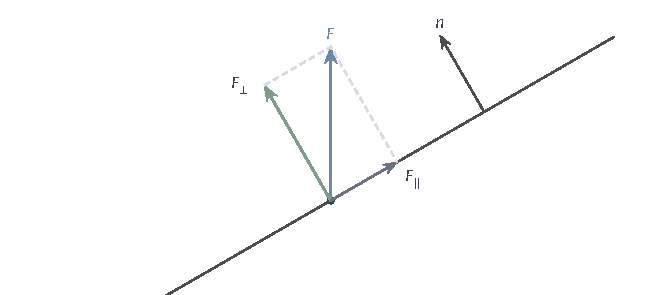
\includegraphics[width=112mm]{figures/01-mathematical-preliminaries-upper/01-mathematical-language-combinatorics-analysis-optimization/tikz/chapter3-concept-processes/normal-projection.pdf}
 \caption{黑斜线表示局部切平面的一个截面，$n$为所选单位法向。向量$F$分为$F_\perp=(F^\top n)n$与切向部分$F_\parallel$；通量使用有符号标量$F^\top n$乘面积，切向部分不贡献。将$n$改为$-n$时标量分量变号，但投影向量$F_\perp$不变，这与直接把场反向不同。}
 \label{fig:analysis-process-normal-projection}
\end{figure}

\paragraph{可积性的要求}

通量只累计法向分量，因此其有限可积性的准确条件是
\[
 \iint_E
 \left|\bm F(\bm r(u,v))^\top(\bm r_u\times\bm r_v)\right|
 \,\mathrm du\,\mathrm dv<\infty.
\]
一个更容易验证的充分条件是$\int_S\lVert\bm F\rVert_2\,\mathrm dS<\infty$。
因为$\lVert\bm n\rVert_2=1$，Cauchy--Schwarz不等式给出
$|\bm F^\top\bm n|\leq\lVert\bm F\rVert_2$。
连续向量场在本节的紧致有限分片曲面上有界，因而满足这一充分条件。
切向分量不进入通量，所以不能把法向分量可积与向量场各分量都可积视为同一个条件。

\subsubsection{积分的性质}

以下运算都在同一曲面、同一法向约定下进行，并假定各法向分量可积。
它们可归结为标量函数$\bm F^\top\bm n$的面积积分，但方向变化需要单独说明。

\paragraph{加法}

向量场相加以后，其法向分量也相加，因此
\[
 \begin{aligned}
 \int_S(\bm F+\bm G)^\top\bm n\,\mathrm dS
 &=\int_S\bm F^\top\bm n\,\mathrm dS\\
 &\quad{}+\int_S\bm G^\top\bm n\,\mathrm dS.
 \end{aligned}
\]
绝对可积性由两项法向分量的绝对值之和控制，积分等式来自标量面积积分的加法性质。

\paragraph{减法}

向量场相减以后，其法向分量也相减，因此
\[
 \begin{aligned}
 \int_S(\bm F-\bm G)^\top\bm n\,\mathrm dS
 &=\int_S\bm F^\top\bm n\,\mathrm dS\\
 &\quad{}-\int_S\bm G^\top\bm n\,\mathrm dS.
 \end{aligned}
\]
两项法向分量绝对可积时，它们的差仍绝对可积，积分等式来自标量面积积分的减法性质。

\paragraph{数乘}

实数$c$可以提出积分号，原因是$(c\bm F)^\top\bm n=c(\bm F^\top\bm n)$，即
\[
 \int_S(c\bm F)^\top\bm n\,\mathrm dS
 =c\int_S\bm F^\top\bm n\,\mathrm dS.
\]
这里缩放的是场，曲面的法向约定保持固定。

\paragraph{曲面分割的可加性}

将$S$分为内部不重叠的有限片$S_1,\ldots,S_N$，并在每片采用原定向的限制，则
\[
 \int_S\bm F^\top\bm n\,\mathrm dS
 =\sum_{j=1}^N\int_{S_j}\bm F^\top\bm n\,\mathrm dS.
\]
零面积接缝不贡献积分；若某片单独反转法向，就改变了被累计的符号，不能仍按同一定向求和。

\paragraph{法向反转}

在场和曲面不变时，把$\bm n$换成$-\bm n$会使通量变号：
\[
 \int_S\bm F^\top(-\bm n)\,\mathrm dS
 =-\int_S\bm F^\top\bm n\,\mathrm dS.
\]

\paragraph{重参数化}

更换参数时，保持已选定的几何法向。重参数化定理表明，参数叉积多出$\det\bm J_T$，
而区域换元使用$|\det\bm J_T|$；若变换翻转参数方向，必须同时校正叉积相对于所选法向的符号。
固定曲面的定向并完成这一校正，通量便与参数选择无关。

\subsubsection{积分的计算}

计算通量时，先固定法向，再选与之相容的参数化，最后累计$\bm F$与有向面积向量的内积。
对于图像曲面$z=\psi(x,y)$，前面已求出叉积$(-\psi_x,-\psi_y,1)^\top$，它的第三分量为正。
因此取向上法向时，对$\bm F=(P,Q,R)^\top$有
\[
 \int_S\bm F^\top\bm n\,\mathrm dS
 =\iint_D(-P\psi_x-Q\psi_y+R)(x,y,\psi(x,y))\,\mathrm dx\,\mathrm dy.
\]
取向下法向则在右侧加负号。这一式直接使用有向面积，不能再额外乘一次叉积长度。

在平面片$\bm r(u,v)=(u,v,u+v)^\top$上，向上单位法向为$(-1,-1,1)^\top/\sqrt3$。
对竖直单位场$\bm F=(0,0,1)^\top$，场与参数叉积的内积为$1$，故
\[
 \int_S\bm F^\top\bm n\,\mathrm dS
 =\int_0^1\int_0^1 1\,\mathrm du\,\mathrm dv=1.
\]
其面积为$\sqrt3$，但法向分量只有$1/\sqrt3$。
同样地，平面$z=ax+by+c$在单位圆盘上方的部分对该场的向上通量为$\pi$，
等于水平投影面积；它的实际面积则为$\pi\sqrt{1+a^2+b^2}$。

对半径$R$的球面，前面采用$(\varphi,\theta)$次序的参数叉积指向外侧。
若$\bm F(\bm x)=\bm x/R$，则球面上的$\bm F$恰等于外单位法向，故
\[
 \int_S\bm F^\top\bm n\,\mathrm dS
 =\int_S1\,\mathrm dS=4\pi R^2.
\]
内向通量为$-4\pi R^2$。这次面积与外向通量相等，是因为法向分量处处为$1$；
下一节再用空间区域内部的散度累计核对同一个通量。

\FloatBarrier
